\section{Calibrating the test}
\label{sec:calib}

The sea-ice benchmark cannot establish sensitivity, because the crop-dependence of
that pipeline is the unknown being estimated. So we built a labeller with a dial. Sen1Floods11~\cite{bonafilia2020sen1floods11}
ships an Otsu-on-VH~\cite{otsu1979threshold} label set computed once per chip, whose
preprocessing we recover in \Cref{sec:recovery}. Holding that smoothing at the chip
level and recomputing only the threshold inside each crop reproduces the sea-ice
mechanism with one scalar per crop as the entire source of crop-dependence:
\begin{equation}
\tau_c(\alpha) = (1-\alpha)\,\tau_{\text{chip}} + \alpha\,\tau_{\text{crop}} .
\label{eq:dial}
\end{equation}
At $\alpha = 0$ the labels are crop-invariant by construction. At $\alpha = 1$ the
labeller is fully closed-loop. The measured spread of per-crop thresholds within a
chip is 6.13\,dB, so the dial has real range.

The artefact set is fixed at the $\alpha = 1$ labels and every arm is scored on
those same pixels. Without that, the artefact set would shrink as $\alpha$ fell and vanish at
$\alpha = 0$, leaving the control with no pixels to be null on. The sea-ice control
works the same way, evaluating a scene-trained model against the original labels.

\begin{figure}[tb]
\centering
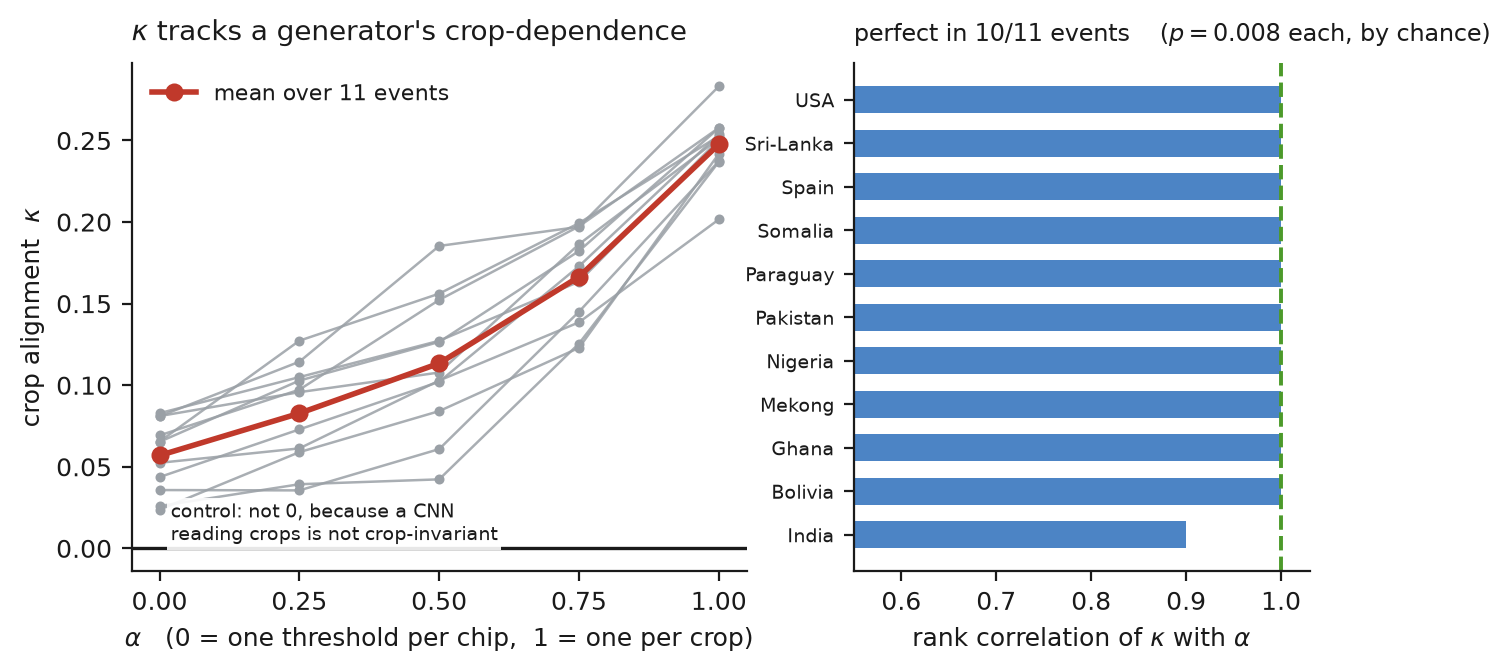
\includegraphics[width=\linewidth]{figures/controlled_calibration.png}
\caption{$\kap$ against the dial of \cref{eq:dial}. Grey lines are held-out events,
red is the mean. Right: rank correlation of $\kap$ with $\alpha$ per event.}
\label{fig:calib}
\end{figure}

\begin{table}[tb]
\centering
\small
\setlength{\tabcolsep}{4pt}
\begin{tabular}{lccccc}
\toprule
$\alpha$ & 0.00 & 0.25 & 0.50 & 0.75 & 1.00 \\
\midrule
$\kap$   & $+0.0569$ & $+0.0828$ & $+0.1134$ & $+0.1664$ & $\mathbf{+0.2476}$ \\
$\Omega$ & 0.0807 & 0.0841 & 0.0897 & 0.0977 & 0.1135 \\
\bottomrule
\end{tabular}
\caption{Crop alignment and model crop-dependence against the dial of
\cref{eq:dial}, averaged over the eleven held-out events.}
\label{tab:calib}
\end{table}

\cref{tab:calib} and \cref{fig:calib} give the result. The contrast between the ends
is $+0.1907$ (sd $0.0212$, $t = 29.84$), positive in 11 of 11 events, sign test
$p = 0.00098$. Per-event rank correlation with $\alpha$ averages $+0.991$ and is
perfect in 10 of 11 events. The exception is a $0.0002$ inversion at the floor
between $\alpha = 0$ and $\alpha = 0.25$.

Positivity on closed-loop labels alone could be accidental. Reproducing the
ordering across five settings, within each event, is harder to get by accident: a
single event ordering five levels correctly by chance has $p = 1/120$.

\paragraph{Scope.} Sen1Floods11 as published computes one threshold per chip, so the
closed-loop artefact is not present in that benchmark. The imagery and the labeller
are real and the crop-dependence is ours. This is a calibration, not a second
sighting in the wild, and nothing here bears on that dataset's published labels.
